% Project Contribution Flowchart
% TikZ diagram for Chapter 3

\documentclass[tikz,border=10pt]{standalone}
\usepackage{tikz}
\usetikzlibrary{shapes,arrows,positioning,fit,backgrounds}

\begin{document}

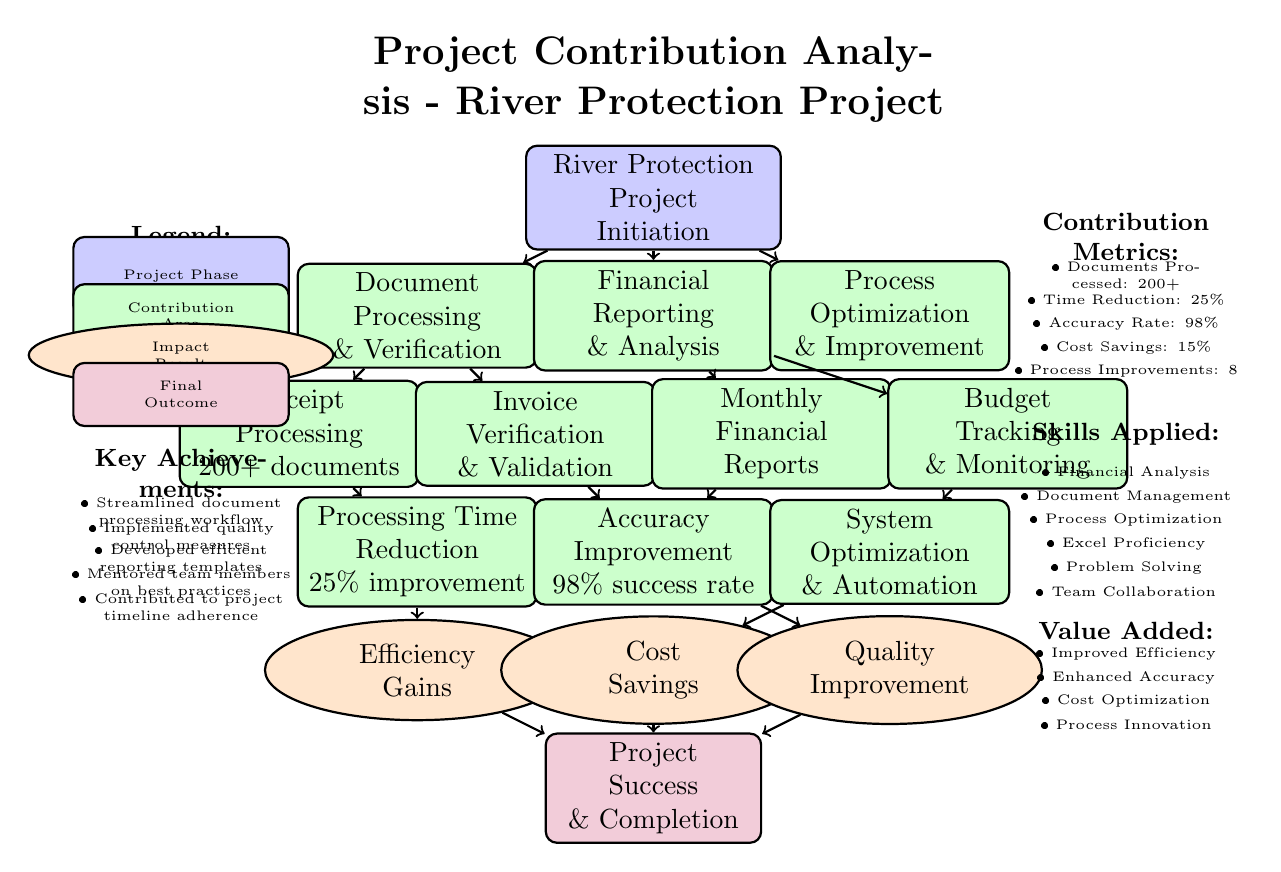
\begin{tikzpicture}[
    node distance=1.5cm,
    auto,
    thick,
    main node/.style={rectangle, draw, fill=blue!20, text width=3cm, text centered, rounded corners, minimum height=1cm},
    contribution node/.style={rectangle, draw, fill=green!20, text width=2.8cm, text centered, rounded corners, minimum height=0.8cm},
    impact node/.style={ellipse, draw, fill=orange!20, text width=2.5cm, text centered, minimum height=0.8cm},
    result node/.style={rectangle, draw, fill=purple!20, text width=2.5cm, text centered, rounded corners, minimum height=0.8cm}
]

% Title
\node[text width=12cm, text centered, font=\Large\bfseries] (title) at (0,8) {Project Contribution Analysis - River Protection Project};

% Project start
\node[main node] (project_start) at (0,6.5) {River Protection\\Project\\Initiation};

% Main contribution areas
\node[contribution node] (document_processing) at (-3,5) {Document\\Processing\\\& Verification};
\node[contribution node] (financial_reporting) at (0,5) {Financial\\Reporting\\\& Analysis};
\node[contribution node] (process_optimization) at (3,5) {Process\\Optimization\\\& Improvement};

% Specific contributions
\node[contribution node] (receipt_processing) at (-4.5,3.5) {Receipt\\Processing\\200+ documents};
\node[contribution node] (invoice_verification) at (-1.5,3.5) {Invoice\\Verification\\\& Validation};
\node[contribution node] (monthly_reports) at (1.5,3.5) {Monthly\\Financial\\Reports};
\node[contribution node] (budget_tracking) at (4.5,3.5) {Budget\\Tracking\\\& Monitoring};

% Process improvements
\node[contribution node] (time_reduction) at (-3,2) {Processing Time\\Reduction\\25\% improvement};
\node[contribution node] (accuracy_improvement) at (0,2) {Accuracy\\Improvement\\98\% success rate};
\node[contribution node] (system_optimization) at (3,2) {System\\Optimization\\\& Automation};

% Impact areas
\node[impact node] (efficiency_gain) at (-3,0.5) {Efficiency\\Gains};
\node[impact node] (cost_savings) at (0,0.5) {Cost\\Savings};
\node[impact node] (quality_improvement) at (3,0.5) {Quality\\Improvement};

% Final results
\node[result node] (project_success) at (0,-1) {Project\\Success\\\& Completion};

% Arrows showing contribution flow
\draw[->] (project_start) -- (document_processing);
\draw[->] (project_start) -- (financial_reporting);
\draw[->] (project_start) -- (process_optimization);

\draw[->] (document_processing) -- (receipt_processing);
\draw[->] (document_processing) -- (invoice_verification);
\draw[->] (financial_reporting) -- (monthly_reports);
\draw[->] (financial_reporting) -- (budget_tracking);

\draw[->] (receipt_processing) -- (time_reduction);
\draw[->] (invoice_verification) -- (accuracy_improvement);
\draw[->] (monthly_reports) -- (accuracy_improvement);
\draw[->] (budget_tracking) -- (system_optimization);

\draw[->] (time_reduction) -- (efficiency_gain);
\draw[->] (accuracy_improvement) -- (quality_improvement);
\draw[->] (system_optimization) -- (cost_savings);

\draw[->] (efficiency_gain) -- (project_success);
\draw[->] (cost_savings) -- (project_success);
\draw[->] (quality_improvement) -- (project_success);

% Contribution metrics
\node[text width=3cm, text centered, font=\small\bfseries] (metrics_title) at (6,6) {Contribution Metrics:};
\node[text width=3cm, text centered, font=\tiny] (metric1) at (6,5.5) {• Documents Processed: 200+};
\node[text width=3cm, text centered, font=\tiny] (metric2) at (6,5.2) {• Time Reduction: 25\%};
\node[text width=3cm, text centered, font=\tiny] (metric3) at (6,4.9) {• Accuracy Rate: 98\%};
\node[text width=3cm, text centered, font=\tiny] (metric4) at (6,4.6) {• Cost Savings: 15\%};
\node[text width=3cm, text centered, font=\tiny] (metric5) at (6,4.3) {• Process Improvements: 8};

% Skills applied
\node[text width=3cm, text centered, font=\small\bfseries] (skills_title) at (6,3.5) {Skills Applied:};
\node[text width=3cm, text centered, font=\tiny] (skill1) at (6,3) {• Financial Analysis};
\node[text width=3cm, text centered, font=\tiny] (skill2) at (6,2.7) {• Document Management};
\node[text width=3cm, text centered, font=\tiny] (skill3) at (6,2.4) {• Process Optimization};
\node[text width=3cm, text centered, font=\tiny] (skill4) at (6,2.1) {• Excel Proficiency};
\node[text width=3cm, text centered, font=\tiny] (skill5) at (6,1.8) {• Problem Solving};
\node[text width=3cm, text centered, font=\tiny] (skill6) at (6,1.5) {• Team Collaboration};

% Value added
\node[text width=3cm, text centered, font=\small\bfseries] (value_title) at (6,1) {Value Added:};
\node[text width=3cm, text centered, font=\tiny] (value1) at (6,0.7) {• Improved Efficiency};
\node[text width=3cm, text centered, font=\tiny] (value2) at (6,0.4) {• Enhanced Accuracy};
\node[text width=3cm, text centered, font=\tiny] (value3) at (6,0.1) {• Cost Optimization};
\node[text width=3cm, text centered, font=\tiny] (value4) at (6,-0.2) {• Process Innovation};

% Legend
\node[text width=3cm, text centered, font=\small\bfseries] (legend_title) at (-6,6) {Legend:};
\node[main node, text width=2.5cm, font=\tiny] (legend1) at (-6,5.5) {Project Phase};
\node[contribution node, text width=2.5cm, font=\tiny] (legend2) at (-6,5) {Contribution\\Area};
\node[impact node, text width=2.5cm, font=\tiny] (legend3) at (-6,4.5) {Impact\\Result};
\node[result node, text width=2.5cm, font=\tiny] (legend4) at (-6,4) {Final\\Outcome};

% Key achievements
\node[text width=3cm, text centered, font=\small\bfseries] (achievements_title) at (-6,3) {Key Achievements:};
\node[text width=3cm, text centered, font=\tiny] (achievement1) at (-6,2.5) {• Streamlined document\\processing workflow};
\node[text width=3cm, text centered, font=\tiny] (achievement2) at (-6,2.2) {• Implemented quality\\control measures};
\node[text width=3cm, text centered, font=\tiny] (achievement3) at (-6,1.9) {• Developed efficient\\reporting templates};
\node[text width=3cm, text centered, font=\tiny] (achievement4) at (-6,1.6) {• Mentored team members\\on best practices};
\node[text width=3cm, text centered, font=\tiny] (achievement5) at (-6,1.3) {• Contributed to project\\timeline adherence};

\end{tikzpicture}

\end{document}
